\documentclass[aspectratio=169]{beamer}

% Custom theme and packages
\usepackage{beamertheme-custom}
% Custom symbols and commands
\usepackage{symbols-custom}

\graphicspath{{figures/}}


\title{Cognitive psychometrics: ethical considerations}
\author{Joachim Vandekerckhove}
\date{Spring 2025}

\titlegraphic{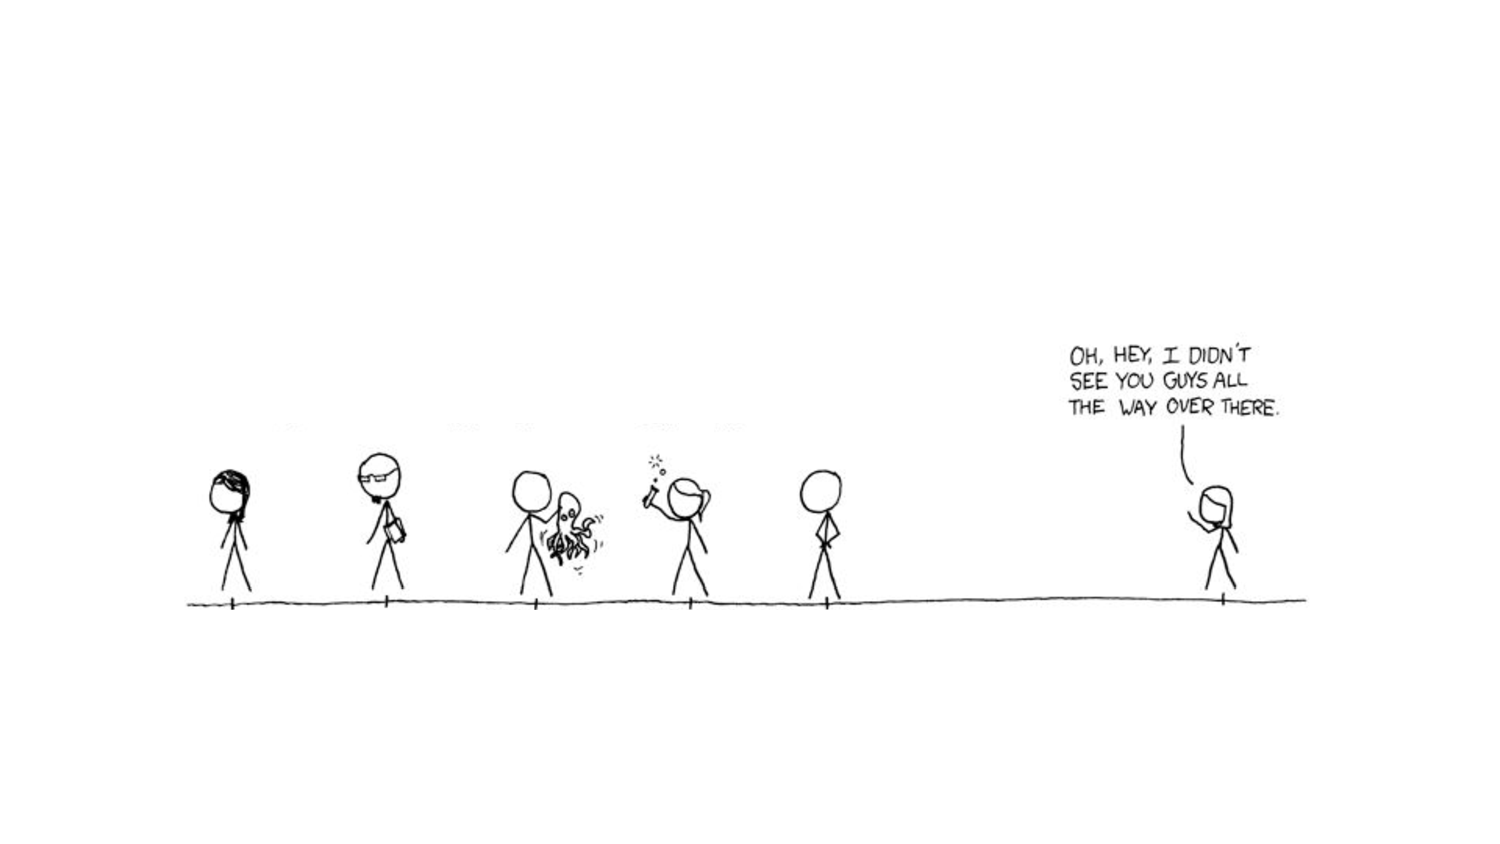
\includegraphics[scale=.625,clip,trim=-10pt 0pt 0 -50pt]{../figures/purity.pdf}}

% Font
\usefonttheme[onlymath]{serif}

\begin{document}

\maketitle

% --- Introduction ---
\begin{frame}{Psychometrics and ethics}
  \begin{itemize}
    \item Psychometrics is the science of psychological measurement (intelligence, personality, aptitude)\pause
    \item Cognitive science provides tools for studying individual differences, underpinning research, diagnosis, and educational assessment\pause
    \item Psychometric tools impact lives\pause
    \item Requires serious ethical scrutiny\pause
    \item Easily abused by scientific racists, eugenicists, and other pseudoscientists
  \end{itemize}
\end{frame}


% --- Historical Ethical Failures ---
\section{The shadow of the past}

\begin{frame}{The allure of quantification}
  \begin{itemize}
    \item Late 19th/early 20th century: drive to establish psychology as a ``hard science.''\pause
    \item Early tools to quantify mental faculties reflected societal biases of the era.\pause
  \end{itemize}
  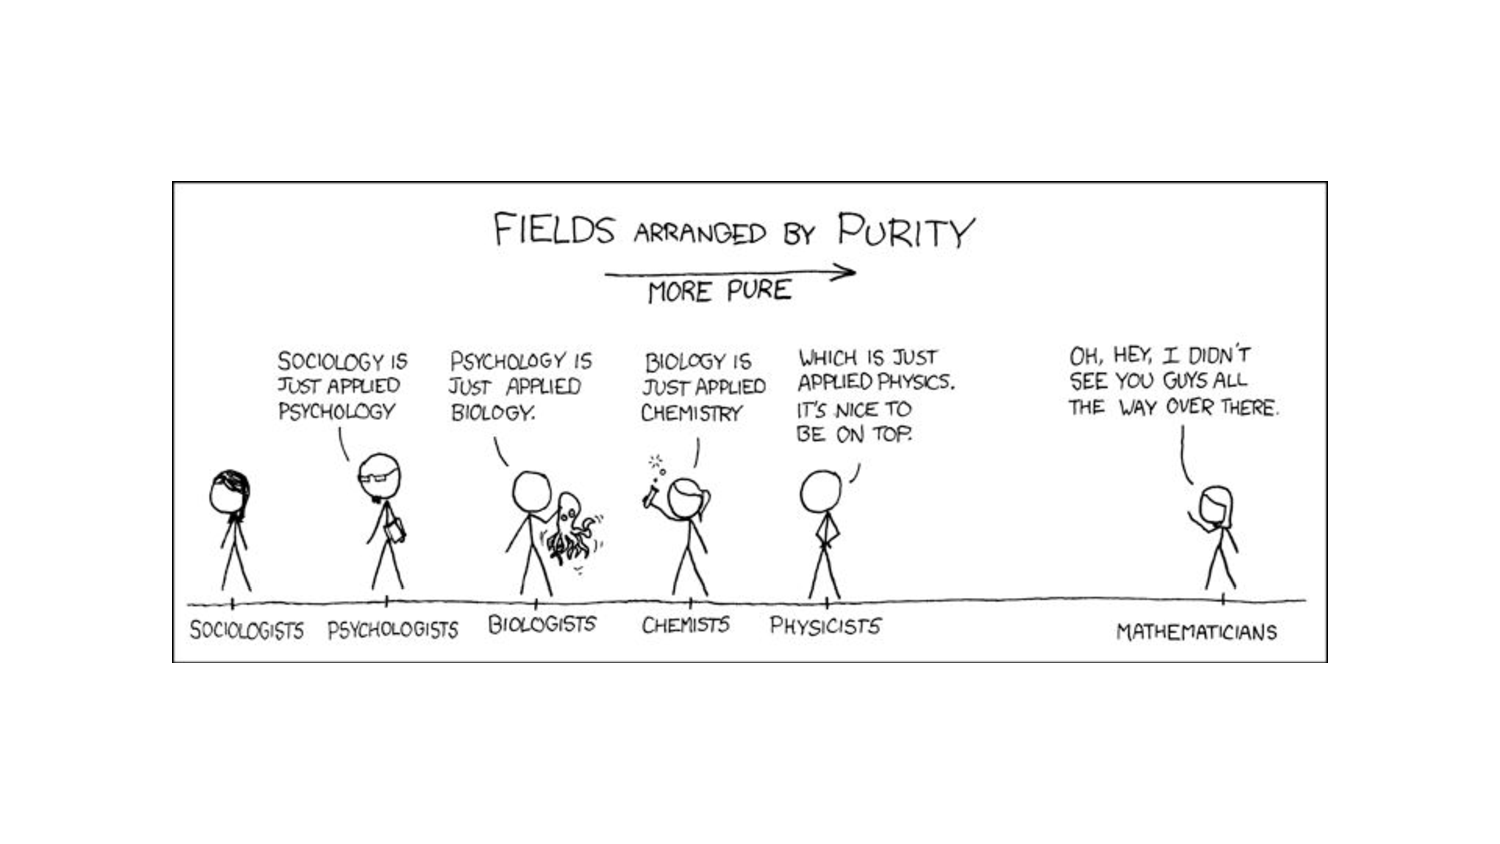
\includegraphics[width=\textwidth,clip,trim=0 50pt 0 70pt]{../figures/purity-full.pdf}
\end{frame}

\begin{frame}{Scientific racism and eugenics}
  \begin{itemize}
    \item Both are based on the idea that certain groups are inferior to others in some sense.
    \item You can ``prove'' all sorts of inferiority/superiority claims if you are willing to cherry-pick data or take invalid liberties with measurement and statistics.
  \end{itemize}
  \vbox to 6cm{
  \only<1>{\begin{definition}[Scientific racism]
    Use of pseudoscientific practices and claims to justify racial hierarchies or discrimination. Measurement of skull sizes (phrenology) within and between populations was used to conclude that some races are inherently less intelligent.
  \end{definition}}
  \only<2>{\begin{definition}[Eugenics]
    The belief or practice of improving the genetic quality of the human population through selective breeding or sterilization.  Some governments have enacted policies to sterilize individuals deemed ``unfit'' to reproduce (e.g., based on mental health diagnoses), and make health care more easily accessible for certain subpopulations than others, etc.
  \end{definition}}
  \vfill
}
\end{frame}

\begin{frame}{Case study 1: eugenics and intelligence testing}
  \begin{itemize}
    \item Key figures: Galton, Goddard, Terman, Brigham.\pause
    \item Misuse of early IQ tests to argue for intellectual inferiority of certain racial/ethnic groups and the ``feeble-minded.''\pause
    \item \textbf{Consequences:} discriminatory immigration policies (e.g., US Immigration Act of 1924), forced sterilization programs.\pause
    \item \textbf{Ethical breaches:} gross cultural bias, lack of validity, confirmation bias, justification for harmful social engineering.\pause
    \item \textbf{Today:} This still just happens, it's not even particularly more subtle (e.g., Richard Lynn's ``The Intelligence of Nations'' was published in 2019; Lynn also argued for sex differences in intelligence).
  \end{itemize}
\end{frame}

\begin{frame}{Case study 2: cultural bias in test development}
  \begin{itemize}
    \item Many early tests normed on specific, often privileged, populations (e.g., white, middle-class).\pause
    \item Test items often reflected specific cultural knowledge, not universal cognitive ability.\pause
    \item \textbf{Consequences:} mislabeling individuals from diverse backgrounds, flawed educational tracking, perpetuation of systemic inequalities.\pause
    \item \textbf{Ethical breaches:} lack of fairness and equity, failure to consider construct-irrelevant variance.
  \end{itemize}
\end{frame}

\begin{frame}{Ethical failures are also scientific failures}
 Many scientific questions are really questions about values\pause
  \begin{itemize}
    \item For example, whether an AI is ``really intelligent'' or ``has consciousness'' is really a question about how we should treat it, whether we should give it rights, etc.\pause
    \item The same is true for classical intelligence testing of people\pause
    \item Very first IQ tests were to determine which children merited which education\pause
    \item We still give different legal rights to people based on their IQ scores
  \end{itemize}
  \pause
  \textbf{Even if that is what you want to do}, tests need to be valid -- they need to \textit{measure what they purport to measure} -- and that has often not been the case.\pause

  (E.g., Lynn's work compared children in remedial education programs to children in regular high schools.)
\end{frame}

\begin{frame}{Other historical ethical issues}
  \begin{itemize}
    \item \textbf{Over-generalization and labeling:} treating scores as definitive, immutable measures of an individual's worth or potential.\pause
    \item \textbf{Lack of informed consent:} individuals often tested without clear understanding of the test's purpose or how results would be used.\pause
    \item \textbf{Transparency issues:} limited access to test content or understanding of scoring for test-takers.
  \end{itemize}
\end{frame}

% --- Contemporary Ethical Challenges ---
\section{Contemporary ethical challenges}

\begin{frame}{Transition: lessons learned or repeated?}
  \begin{itemize}
    \item While the field has evolved, many historical concerns persist in new forms.\pause
    \item New technologies also introduce novel ethical dilemmas.\pause
    \item Any number of computer image processing studies are basically phrenology (physiognomy).
  \end{itemize}
  \begin{center}
    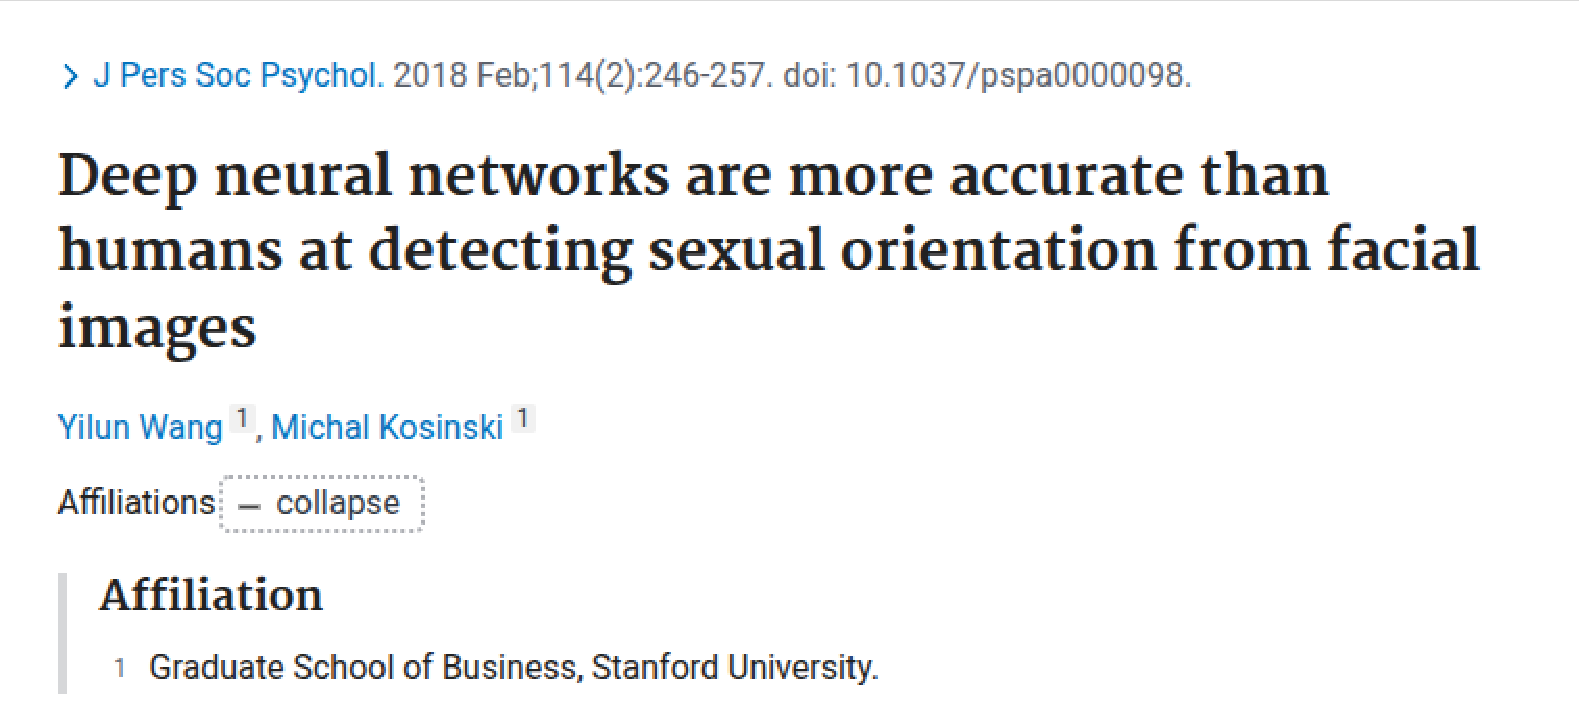
\includegraphics[scale=.4]{../figures/kosinski.pdf}
  \end{center}
\end{frame}

\begin{frame}{Fairness, equity, and bias today}
  \begin{itemize}
    \item Ensuring tests are fair across diverse cultural, linguistic, and socioeconomic groups remains a major challenge.\pause
    \item Tools like differential item functioning (DIF) analysis help detect bias.
    $$\theta_{pi} = \beta_0 + \beta_A \times \text{Ability}_p + \beta_G \times \text{Group}_p \times \text{DIF}_{Gi} + \varepsilon_p$$\pause
    \item Challenges in test translation and cross-cultural adaptation.
  \end{itemize}
\end{frame}

\begin{frame}{Informed consent and test user competence}
  \begin{itemize}
    \item Test-takers (or guardians) must understand:\pause
    \begin{itemize}
        \item Purpose and nature of the test.\pause
        \item How results will be used and their limitations.\pause
        \item Rights (e.g., to receive feedback, refuse testing in some contexts).\pause
    \end{itemize}
    \item Critical for vulnerable populations (minors, patient groups, the incarcerated).\pause
    \item \textbf{Common ethical principles:} autonomy, beneficence, non-maleficence.
  \end{itemize}
\end{frame}

\begin{frame}{High-stakes testing}
  \begin{itemize}
    \item Major life decisions (admissions, employment, licensure) remain heavily reliant on single test scores.\pause
    \item Potential for ``teaching to the test,'' (e.g., SAT prep), anxiety, narrowing of curricula.\pause
    \item Balancing test utility with potential for individual and societal harm.\pause
    \item \textbf{Ethical principle:} justice, scrutiny of consequences.
  \end{itemize}
\end{frame}

\begin{frame}{Big data and machine learning in assessment}
  \begin{itemize}
    \item Large-scale collection of behavioral and performance data\pause
    \item Privacy concerns with data aggregation and sharing\pause
    \item Potential for automated profiling and discrimination\pause
    \item Risk of reinforcing existing societal biases\pause
    \item Need for transparency in algorithmic decision-making
  \end{itemize}
\end{frame}

\begin{frame}{The rise of AI in psychometrics}
  \begin{itemize}
    \item AI for automated scoring, adaptive testing, profiling from digital footprints.\pause
    \item Risk of \textbf{algorithmic bias}: AI learning and amplifying existing societal biases present in training data.\pause
    \item The ``black box'' problem: lack of transparency in AI-driven assessment decisions.
  \end{itemize}
\end{frame}

% --- Towards Ethical Practice ---
\section{Ethical measurement practice}

\begin{frame}{A responsible path}
  \begin{itemize}
    \item The field of psychometrics actively works to address ethical concerns.\pause
    \item This involves professional guidelines, rigorous standards, and ongoing research.\pause
    \item There is a lot of work left to do.\pause
    \item Cognitive modelers need to keep track.
  \end{itemize}
\end{frame}

\begin{frame}{Test development and validation}
  \begin{itemize}
    \item Rigorous validation for specified purposes and populations is crucial.\pause
    \item Continuous research into bias detection and reduction methodologies.\pause
    \item Promoting transparency in test development and scoring processes.
  \end{itemize}
\end{frame}

\begin{frame}{Your role: critical consumer and future professional}
  As cognitive scientists, you may use, develop, or critique psychometric tools.\pause
  
  It is \textbf{your job} to critically evaluate claims made about tests and their uses:\pause
  \begin{itemize}
    \item If you develop a test or measurement tool, consider if it measures what it claims to measure \textit{even outside the context of your studies}?\pause
    \item Understand the limitations inherent in any measurement instrument.\pause
    \item Advocate for ethical practices and consider societal impact of your contributions and omissions.
  \end{itemize}
\end{frame}

\maketitle

\end{document}